\begin{flushleft}
    \normalsize
    \section{Technical Design}

    \subsection{Programming Language Selection and Libraries Used}

    I selected C# as my programming language for several reasons. Currently, it is the language that I am most familiar with. In addition, I conducted research on which languages are best for fast processing, and found that C, C++, and C# are among the top contenders. Considering my skill set and the importance of speed in this situation, I concluded that C# would be a good fit. Furthermore the object orientated nature of the language means that I will be able to separate the front end and the back end processing into separate bll files keeping the code clean and easily maintainable.\\ 
    \bk
    Find below a list of all libraries I used: \\
    
    \subsubsection{Linq}
    In order to manipulate lists and create the data structures that I need I will need to use some Linq methods. During the prototyping stage I found that using some Linq methods such as the Select statement allowed the program to be easier to read and make logical sense. As well as this there have been optimisations made in the iterative Linq methods which will make my program faster. Similar to some of the following libraries this is a Microsoft Library which is open source.
    \\ \bk


    \subsubsection{Bitmap}
    In order for my program to function a required part of it is that it is able to take an image as an input. In native C# there is no set way to do this. Therefore I needed to use the Microsoft System.Drawing Namespace. This namespace provides access to GDI+ basic graphics functionality. This does limit this project as is to only working on Windows since the library requires access to the GDI+ native library which is only on windows services. \\
    
    The only part of this library I will be using is the Bitmap class. This will allow me to accept all types of images without the need of parsing them myself since this is not the aim of my project. 
    \\ \bk

    \subsubsection{Windows Forms}
    In order to complete my objectives my program will need to be easy to use and any user with some degree of technical competency should be able to use it. In order to achieve this objective I though that instead of using some form of console input in order to get a starting and an end location, that it would be better to use some form of GUI. In order to do this I will use Windows Forms. This will allow me to make a simple GUI which will allow the end user to interact with the user and easily understand. \\ 

    The things which I will end up using the windows forms are the map traversal, allowing the user to select a start and an end node with a click instead of having to enter a coordinate. As well as this I will also use forms to show the user the stages of, for example, the canny edge detection.
    \\ \bk

    \subsection{High Level Overview}
    The general purpose of my project is to allow a user to take a map and input it into my program, then subsequently convert it into a routable map. \\ \bk
    
    In order to achieve this goal my program will first take an input, the users map. It will then take this map and convert it into an machine readable format, a Bitmap. Canny edge detection will then be performed on it causing the edges and the surroundings of the paths on the image to be found. Using these edges a filling algorithm will fill the spaces encapsulated by the lines. Finally these filled spaces will be used to convert the whole image to a graph which can then be traversed using graph traversal algorithms such as A* or Dijkstra's algorithm. \\ \bk

    \begin{figure}[H]
        \centering
        \subfloat[\centering High Level Overview Of Program]{{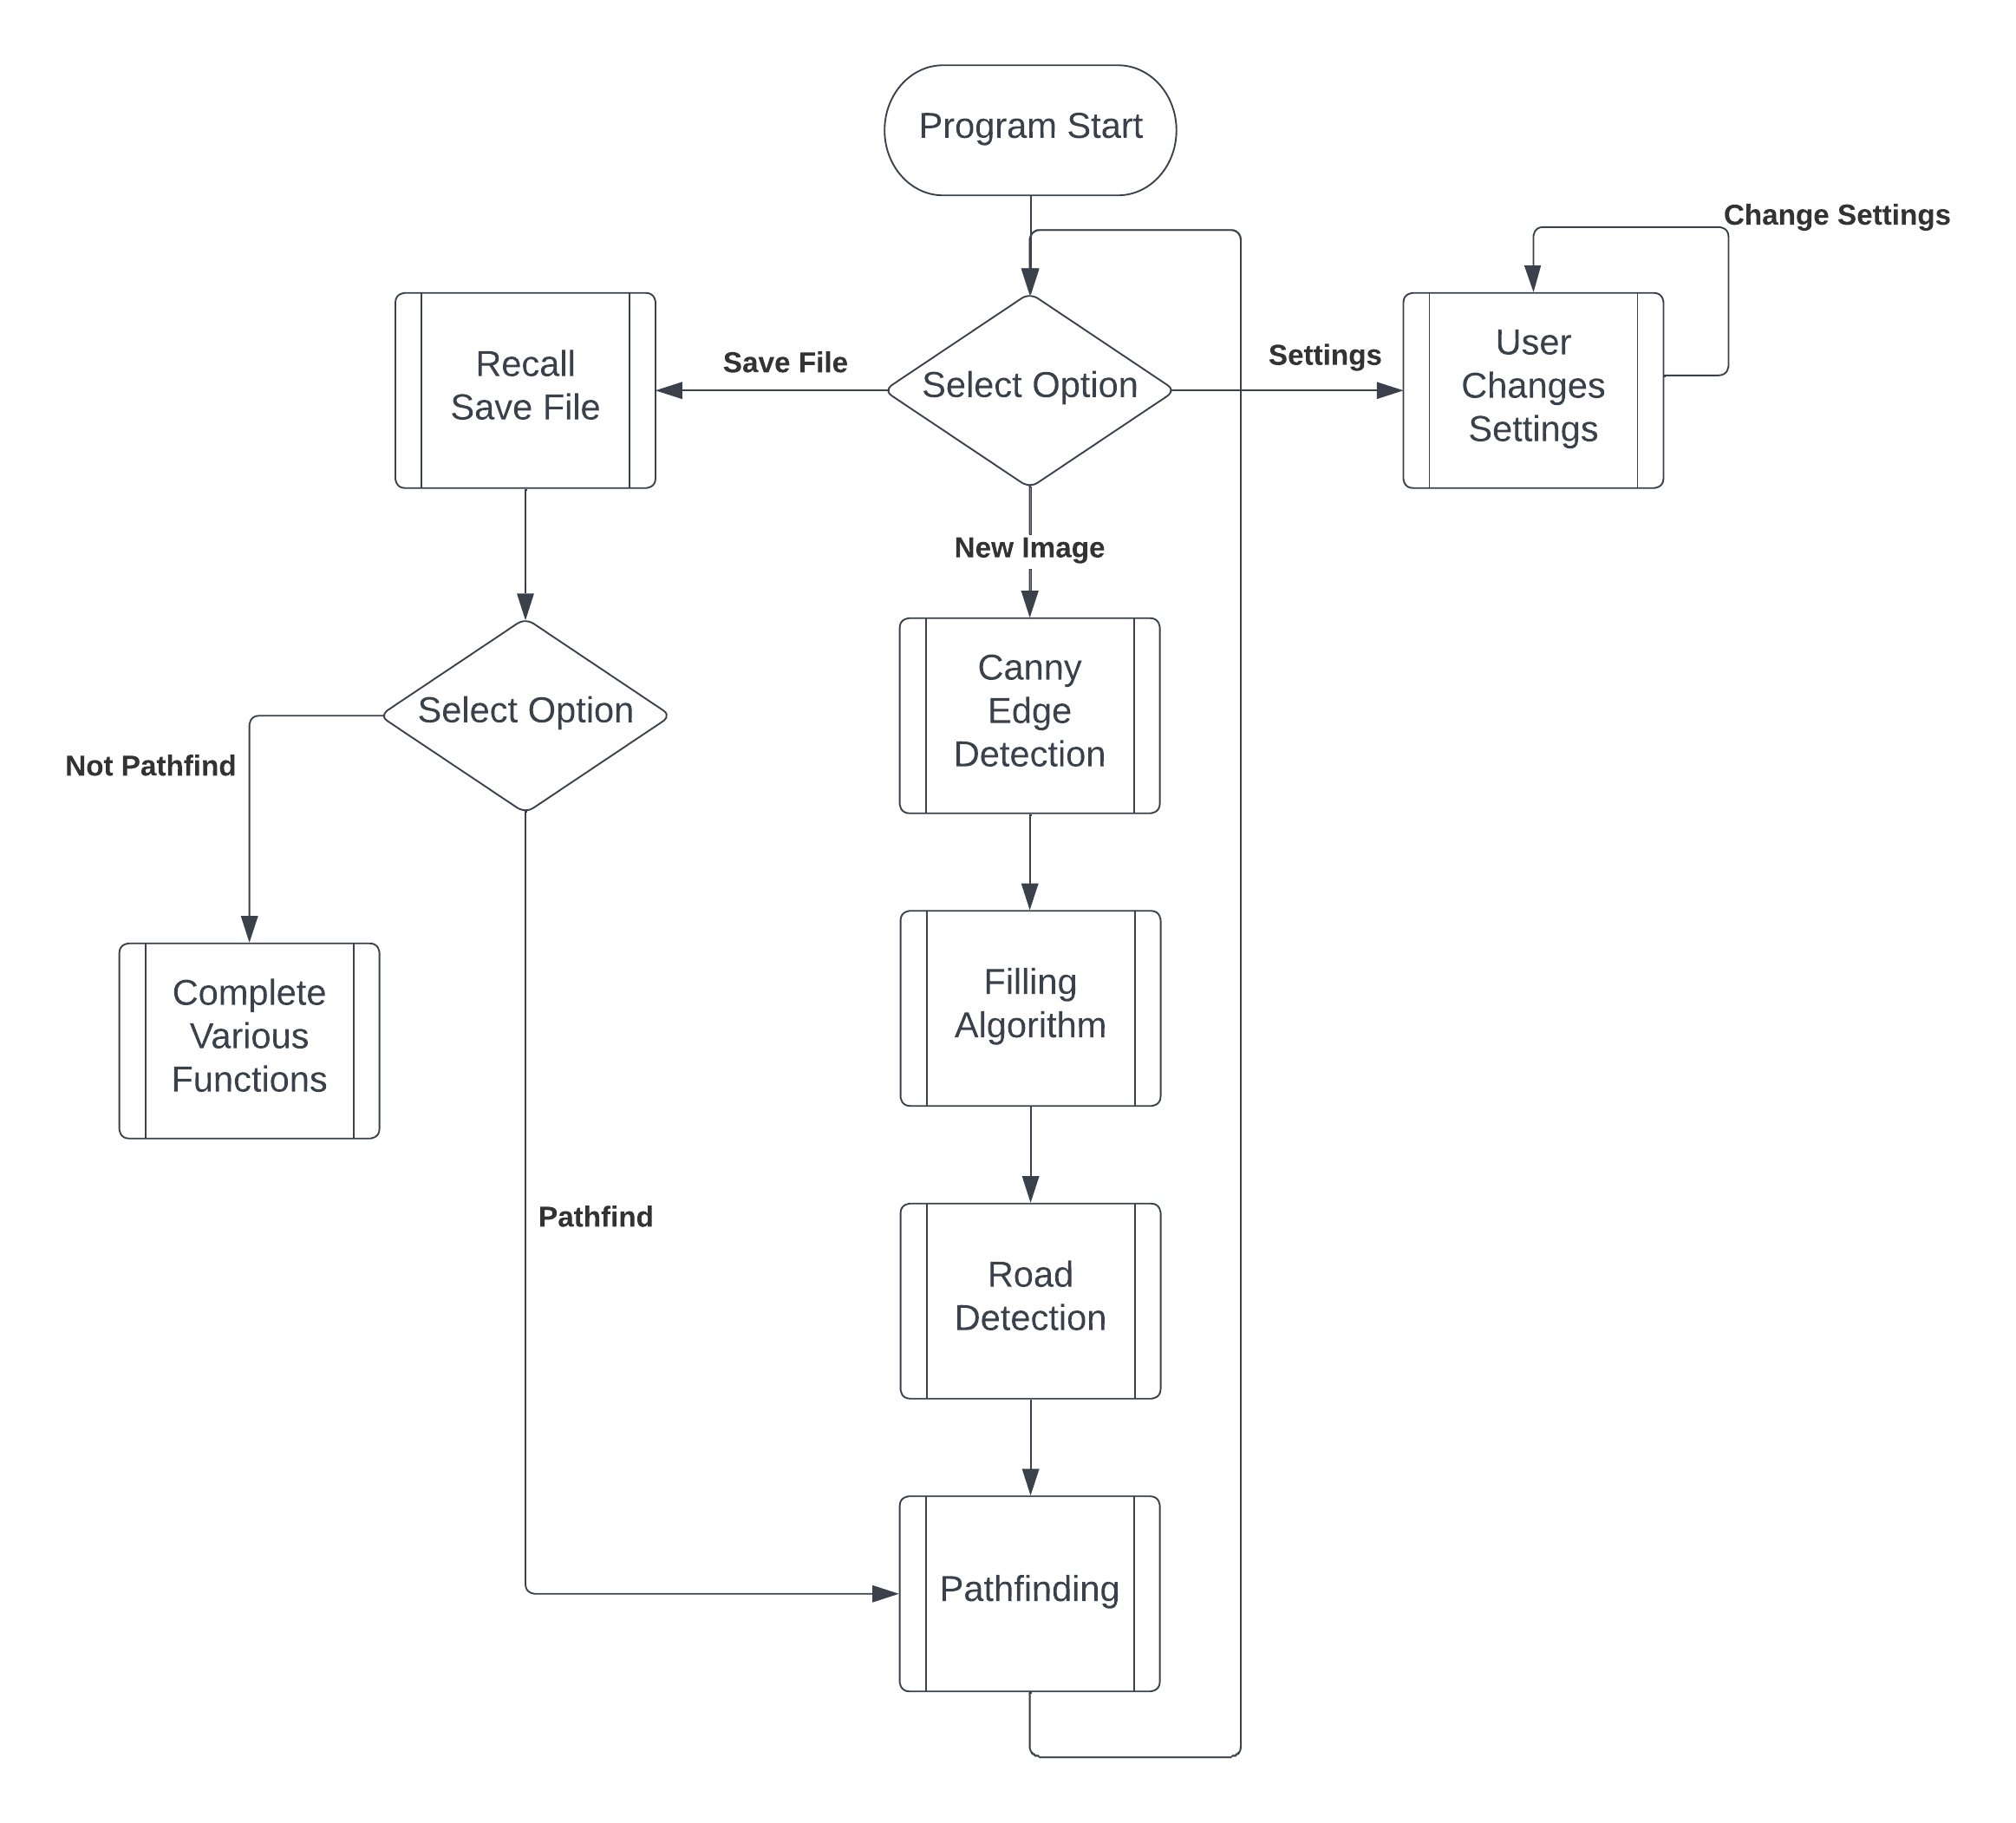
\includegraphics[width=17cm]{images/HighLevelOverview.png}}}
        \caption*{A High Level Overview of the Whole Program}
    \end{figure}

    The version of Edge Detection I will be using as previously stated will be Canny Edge Detection, this is as opposed to Sobel Edge Detection. The main version of filling I will be using is flood fill due to it simple nature to implement ad due to the fact that it does not take much memory and can be made recursive so it performs well. The final main algorithm I will need to use is image kernels and convolution, this will allow me to manipulate the inputted image.

    \subsubsection{Bitmap}
    In order for my program to function a required part of it is that it is able to take an image as an input. In native C# there is no set way to do this. Therefore I needed to use the Microsoft System.Drawing Namespace. This namespace provides access to GDI+ basic graphics functionality. This does limit this project as is to only working on Windows since the library requires access to the GDI+ native library which is only on windows services. \\
    
    The only part of this library I will be using is the Bitmap class. This will allow me to accept all types of images without the need of parsing them myself since this is not the aim of my project. 
    \\ \bk 


\end{flushleft}